\documentclass{beamer}
%
% Choose how your presentation looks.
%
% For more themes, color themes and font themes, see:
% http://deic.uab.es/~iblanes/beamer_gallery/index_by_theme.html
%
\mode<presentation>
{
  \usetheme{boxes}      % or try Darmstadt, Madrid, Warsaw, ...
  \usecolortheme{seahorse} % or try albatross, beaver, crane, ...
  \usefonttheme{serif}  % or try serif, structurebold, ...
  \setbeamertemplate{navigation symbols}{}
  \setbeamertemplate{caption}[numbered]
} 

%%%%%%El Señor Español%%%%%%%%%%%%%%%%%%%%%%%%%%%
\usepackage[utf8]{inputenc} %acento
\usepackage[
spanish, %El lenguaje.
es-tabla, %La tabla y no cuadro.
activeacute, %El acento.
es-nodecimaldot %Punto y no coma con separador de números
]{babel}

\usepackage[utf8]{inputenc}
\usepackage[T1]{fontenc}

\title[Avance]{``Avance'': Tesis de Maestría en Ciencias Físicas}
\author{Evelyn Coronel}
\institute{Partículas y Campos - Centro Atómico Bariloche}
%\date{Date of Presentation}

\begin{document}

\begin{frame}
  \titlepage
\end{frame}

% Uncomment these lines for an automatically generated outline.
%\begin{frame}{Outline}
%  \tableofcontents
%\end{frame}

\section{Introducción}

\begin{frame}{Introducción}

\begin{itemize}
  \item Cosas que hice en la tesis de licenciatura.
  \begin{itemize}
  	\item[-] Corrección del clima
  	\item[-] Familiarizarse con el dataset
  \end{itemize}
  \item Resultados a los que llegué.
  \item Nos movimos a otros tipos de disparos
\end{itemize}

\vskip 1cm

%\begin{block}{Examples}
%Some examples of commonly used commands and features are included, to help you get started.
%\end{block}

\end{frame}

\section{Update}

\begin{frame}{Update}

  \begin{itemize}
  	\item Diferencias con el disparo tradicional.
  	\item Cuestiones con los pesos de los hexágonos.
  	\item Resultados con el rango de energía 1 EeV - 2 EeV.
  \end{itemize}


\end{frame}

\subsection{Update}


\begin{frame}{Pesos}

\begin{figure}[htbp]
	\centering
	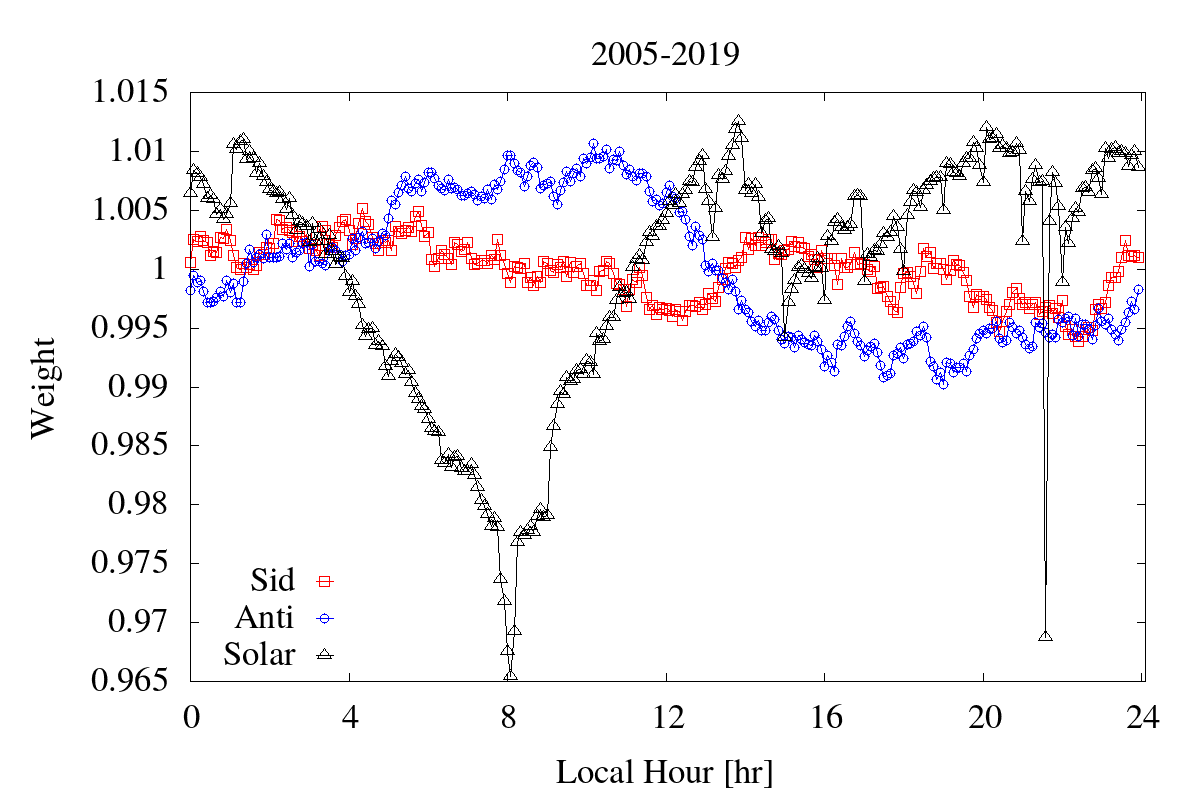
\includegraphics[width=0.95\textwidth]{./../../Cpp/Anisotropy/Report/weigth2005-2019.png}
	\caption{Pesos de los hexágonos en el rango 2005-2019 para distintas frecuencias.}
\end{figure}

\end{frame}

\begin{frame}{Pesos}

\begin{figure}[htbp]
	\centering
	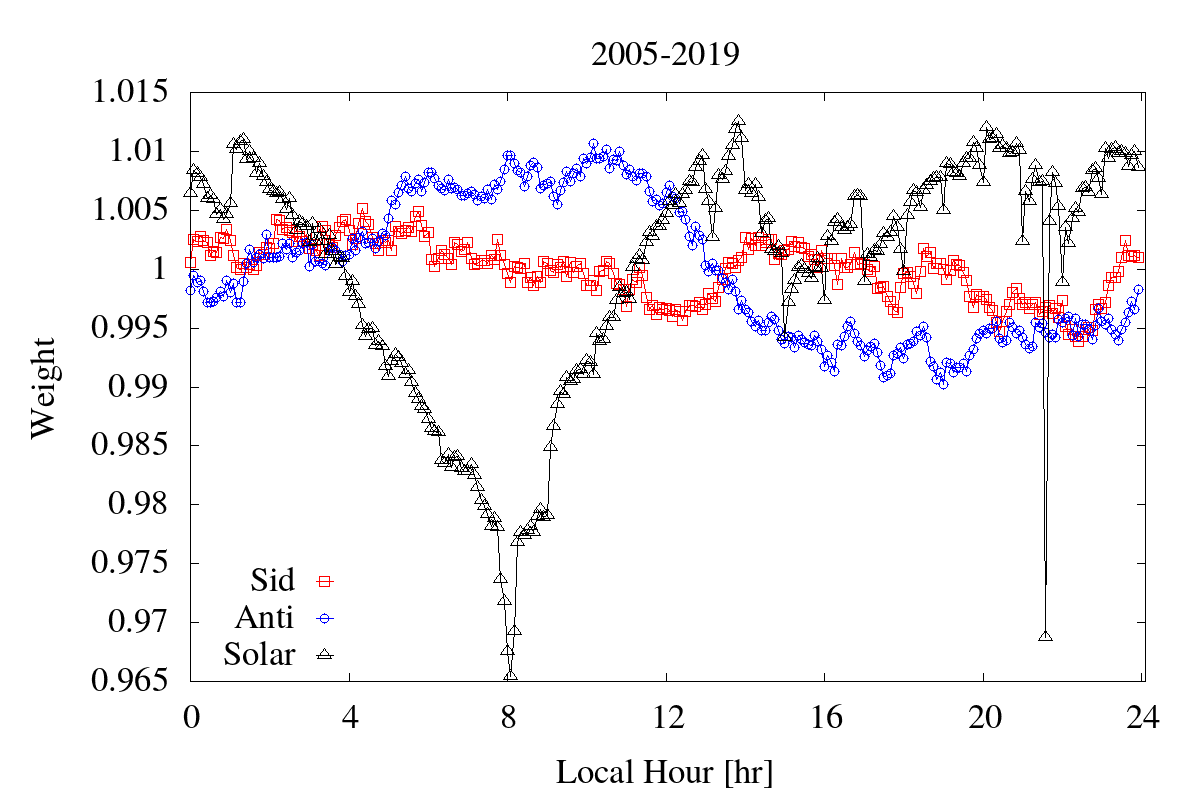
\includegraphics[width=0.95\textwidth]{./../../Cpp/Anisotropy/Report/weigth2005-2019.png}
	\caption{Pesos de los hexágonos en el rango 2005-2019 para distintas frecuencias.}
\end{figure}

\end{frame}

\end{document}